\problemname{\problemyamlname}

\illustration{0.3}{beer-pong.jpg}{
    
    CC BY-SA 4.0 by Suprakon jutasuwan on \href{https://www.vecteezy.com/vector-art/15846056-plastic-cups-vector-red-beer-pong-plastic-cups-with-ball-traditional-drinking-game-vector-illustration}{Vecteezy}
}

% optionally define variables/limits for this problem
\newcommand{\maxn}{10^{6}}

Vous êtes à la finale de la compétition de beer pong du Bénélux. Ce beer pong est un peu différent de celui que vous connaissez. Dans celui-ci tout les verres sont alignés et espacés d'un distance $x_i$ (en mètres), vous voulez boire le plus de verres possible. Vous jouez aussi avec une balle un peu spéciale. C'est une balle qui fait des rebonds de distance constante en fonction de la force avec laquelle vous la lancez.
C'est votre tour, vous avez une balle et vous devez choisir la force avec laquelle vous la lancez. Cependant il est impossible de lancer la balle avec une force inférieure ou égale à 1 étant donné que çà demandrait une concentration hors-normes. Vous voulez maximiser le nombre de verres que vous buvez. Pouvez-vous trouver la force optimale pour maximiser le nombre de verres que vous buvez ?
\smallskip
\begin{figure}[h]
    \centering
    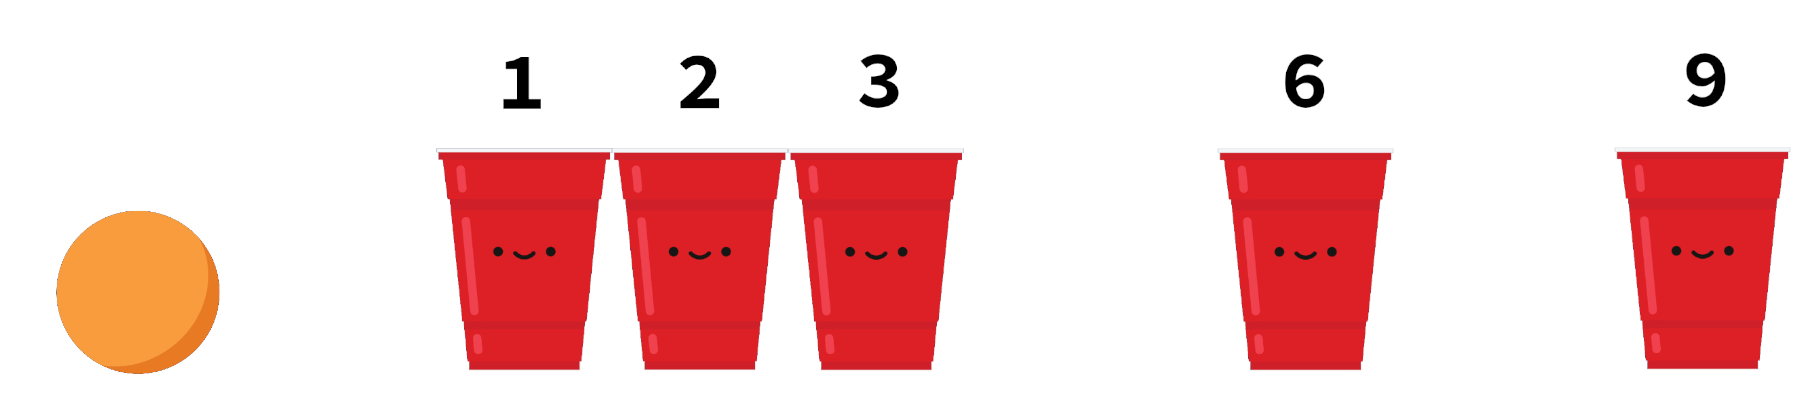
\includegraphics[width=0.7\textwidth]{illustration.png}
    \caption{Example du sample 1}
\end{figure}

\begin{Input}
    L'entrée consiste en:
    \begin{itemize}
        \item Une ligne avec un entier  $n$ ($1\leq n\leq \maxn$), le nombre de gobelet - 1.
        \item $n$ lignes avec un entier $x_i$ ($1\leq x_i\leq \maxn$), la distance entre les verres $i$ et $i+1$. À noter que le lanceur se trouve à la position 0 et que la première distance représente la distance entre le lanceur et le verre 1.
    \end{itemize}
    Il est garantis que la somme des $x_i$ est $\leq 10^6$.
\end{Input}

\begin{Output}
    Sortez la force avec laquelle vous devez lancer la balle pour maximiser le nombre de verres que vous buvez. Ainsi que le nombre de verres que vous buvez.
\end{Output}
